%************************************************
\chapter{Gamified Designs to Drive Consumer-Laborer Alliance}\label{proposal} 

In Chapter \ref{3codesign}, our policymaker participants called for a shifted public perception of gig workers, one that overcome cultural stigmas as well as legal misclassifications.
While Gig2Gether (Chapter \ref{6gig2gether}) demonstrated the potential of a data-sharing tool to intervene in the current barriers obstructing information exchange among workers (and possibly policymakers), the perceptions of consumers remain one influential player of the worker-platform-client triangulation that we have yet to explore. Consumers shape worker conditions in significant ways, through expectations of service quality and pricing \cite{influence}, ratings \cite{homecare} and scaled collective political power \cite{triangle}.
But despite their influence, consumers remain largely unaware of the harsh realities workers face -- Pew Research found that nearly half of Americans have never heard of the ongoing debate around the classification of ridehail drivers \cite{pew}.

Meanwhile, many algorithmic management practices that platforms employ are deliberately opaque and undocumented, obscured from consumer perception and scrutiny. More inconspicuous tactics include (1) psychological strategies like gamification and ratings that manipulatively promote prolonged engagement and surveillance \cite{rating, long_hours, making_out} (2) legal evasions of employer responsibilities and (3) undisclosed and unpredictable wage adjustments that reduce and minimize worker earnings \cite{vasudevangame}. 
A burgeoning body of work engage with workers to expose the hidden and undocumented risks of gig labor, offering worker-centered tools to collectivize and resist \cite{gig2gether, zhang2023stakeholder, homecare}. However, relying primarily on workers to push back against platform tactics and insufficient regulatory infrastructures can add to their vulnerabilities, financially, psychologically and career-wise. Consumers, on the other hand, have more capacity, resources and power to advocate for worker rights and conditions \cite{fastdrink}, but may refrain from broaching and contemplating these sensitive and uncertain topics in casual settings, such as a platform-mediated ride. 

Gamification is one approach to motivate an audience to engage and empathize with serious but sensitive prosocial causes such as gender-based violence \cite{standbyme}, interpersonal racism \cite{provotypes} and HIV prevention \cite{hiv}. Specifically, persuasive game mechanics delivered through means of ``embedded'' messaging or interactive narratives offer players immersive and empathetic spaces where they can learn about or experience driving conditions without being subjected to personally vulnerable positions.
% Taking a more covert and tacit approach, 
This study explores the potentials of game-based interventions as a boundary objects for mediating consumer education and discourse around the obscure and delicate dimensions of rideshare driving conditions. 
Previous works of persuasive games revealed their potential to transform players' attitudes and perceptions on serious social issues, while creating psychological distance between the player and intended message \cite{transformational}. Leveraging techniques and frameworks from persuasive game design, we worked with rideshare drivers and passengers in a series of codesign sessions to explore whether gameplay interventions may transform passengers to understand, empathize towards, and advocate for the obscured realities of rideshare driving.


\begin{enumerate}
\item[\textbf{RQ 1}] 
Which gamified experiences allow effective embedding of ridesharing concepts that drivers desire further advocacy for?

\item[\textbf{RQ 2}] How can such playable interventions motivate consumer engagement and advocacy for the working conditions of rideshare drivers?

\end{enumerate}

% But while workers showed an affinity for the idea of sharing data with policy experts and had ideas for policy initiatives to support that aligned with the receipients of their data (see Chapter \ref{support}), it remains unclear how such (aggregate) data should be presented and visualized. 

% Previous work uncovered how experienced workers developed strategies to cope with the changing nature of platform algorithms \cite{pacify, Jarrahi2019-if}, while more novice workers worked to improve understandings of platforms' underlying algorithmic mechanisms \cite{peersupport}. However, to present understandings on the constantly evolving (but too often unannounced \cite{6B4U}) nature of platform algorithms to the general gig workforce, such insights (currently available online in spaces such as loosely organized forums) require organization and visualization \cite{peersupport}. Thus, I propose investigating potential methods of data visualization that balance curated showcases of grounded experiential worker insights with accurate data aggregations that are digestible and influential to policymaking. 

% Related scholarship also compiled evidence for the effectiveness of tech-enabled collective organization for providing strategic value (i.e., information sharing, collective resource-mobilisation, networking and response generation) in times of community crisis \citep{selforg}. But it is imperative to devise mechanisms for collectivism that anticipate change, in addition to only organizing when responding/reacting to crises. Building upon our nascent approach toward collective worker data-sharng, this chapter also strives to identify modes of (cross-platform and cross-stakeholder) interaction that will best support and incentivize community building, sustainable governance and data-sharing.

\section{Related Works}
\subsection{Labor, Vulnerabilities and Consumer Knowledge Gaps in Rideshare Driving} \label{stressors}
App-based rideshare services have proliferated in the US market since their introduction more than a decade and half ago, emerging as the largest sector of the on-demand economy \cite{making_out}. But while more than 36\% of the US adults used rideshare services \cite{jiang2019more}, Pew Research estimated 43\% of American adults to have never heard about the ongoing debate about the classification of rideshare drivers in 2021, yet those with knowledge of the issue was much more likely (+20\%) to desire further regulation of rideshare companies \cite{pew}. Meanwhile, public opinion surveys show consumers' conflicted opinions about the effects of platform-based gig work for laborers, with especially high ambivalence towards aspects of working conditions that are hidden from their purview -- e.g., long-term consequences on career \cite{triangle}. Consumer perceptions of a platform's working conditions also affect their use and recommendation of it, especially among users with more social consciousness \cite{role}.

Despite increasing concern, there remains a knowledge gap between consumer perceptions of gig work such as rideshare driving and comprehensive understanding of the invisible risks, stressors, and vulnerabilities that drivers and other workers assume \cite{navigating, hazards, distress}, along with unseen immaterial, emotional and logistical labor \cite{immaterial, exploitation}. 
Rating pressures (and their accompanying deactivation thresholds) represent one tactic that platforms leverage to discipline drivers \cite{rating}. 
Such reputational burdens coerce several forms of unpaid emotional labor from drivers, including expectations of maintaining a ``friendly'', ``positive'' and ``respectful'' attitude to please the passenger, regardless of how riders themselves behave \cite{mediatization}.
Despite the objective to satisfy riders, passengers themselves may not be aware of the heavy implications that ratings carry for drivers \cite{immaterial, translating}. 

Workplace gamification is another psychological technique that platforms use to trick and coerce drivers to continue laboring under exploitative conditions \cite{making_out, prabowo2019does, tricks} -- which drivers resist \cite{vasudevangame}. 

Information asymmetries also deprive driver agency when platforms choose to withhold key details of a trip such as exact destination and fare \cite{asymmetries}. The combination of such algorithmic management strategies and the consequences of intense competition (e.g., low wages, social isolation) creates immense psychological stress for drivers \cite{stressfulride, distress} -- who also deal with hidden health and safety risks from accidents on the road \cite{pilot, crashes}, violence from passengers \cite{brush, festering}, fatigue \cite{fatigue} as well as long-term consequences (e.g., musculoskeletal and urinary disorders) \cite{acute, stressfulride}. However, many of these harmful but latent effects remain unobservable to passengers, while more delayed effects may also escape the notice of drivers themselves.

% riders remain unaware of the various forms of immaterial labor \cite{immaterial, exploitation}, psychological stressors as well as invisible risks that plague drivers in everyday operations.

% \begin{itemize}
%     \item studies show how social frictions often exist between drivers and passengers \cite{social}, especially when coming from different age ranges \cite{emails}
%     \item ``How does one value something one cannot and often does not want to see?'' and labor simultaneously as a ``commodity'' and ``lived experience''
%     \item ``hidden curriculum'' of driver responsibilities that doesn't get passed on as in traditional organizations, and which Uber/Lyft try to offload to online driver communities
%     \item potential for riders to crowdsource audits related to algorithmic payment gouging, -- need for indicators
%     \item on-demand transit as a form of disruptive work \cite{on_demand_transit}
% \end{itemize}

\subsection{Technological Advocacy for \& Consumer Perceptions of Rideshare Driving} \label{advocacy_background}
Scholars at the intersection of HCI and labor studies made several attempts to leverage technological probes and interventions to surface and curb the harmful impacts of algorithmic management, as well as to advocate for and design alternative infrastructures that better prioritize driver welling.  \citet{stein2023you} imagined alternative uses of their data and more plural sociotechical infrastructures with drivers to uncover key design objectives surrounding privacy, agency and utility. \citet{zhang2023stakeholder} invited drivers to propose algorithmic imaginaries that offer more worker-centered transpancy, incentives and insights to drive well-being. \citet{alternative} worked with multiple stakeholder groups to reveal need for platform-based changes, technological innovations as well as civic advancements such as more accurate public perceptions of workers. More recent studies stepped beyond co-design to reveal the potential for data probes \cite{zhang2023stakeholder} as well as data-sharing tools \cite{gig2gether, fairfare, bargaining} and collectives \cite{workshop} to advocate and elevate worker priorities and objectives.
But while these approaches demonstrated workers' shared motivations and offered techniques for collective accountability, sensemaking and decision-making, such interactions necessarily require effortful engagement and data contributions from workers, many of whom are locked into laboring for long hours to balance financial needs \cite{good} with instability of job opportunities, making it infeasible for them to engage in additional (uncompensated) interactions. 

Meanwhile, the ways in which rideshare passengers perceive and interact with driving conditions remain relatively underexplored. But more than workers (service providers) or platforms, consumer behavior plays an indispensable role \cite{triangle}. In particular, how consumers perceive the work conditions and quality of a platform's service directly influence their use and recommendation of the provided service \cite{role}, and such perceptions at scale carry immense political power \cite{sceptics}, which platforms seek to influence. Recognizing their foundational role, \citet{triangle} raises the question of whether workers can ``gain support from consumers they serve, altering the power in this triadic relationship?'' In the space of food delivery, \citet{fastdrink} began probing this space by prototyping an interaction that provided users with their courier's demographic information during waiting time, which shifted users away from affective empathy, but toward compassionate empathy -- an experience that incentivizes further prosocial actions to help others \cite{compassion}. 
But while technology-mediated interactions show promise for fostering users' interpersonal empathy for individual workers, it remains unclear whether they hold the potential to cultivate consumer empathy in a way that motivates them to further care, take action and advocate for vulnerabilities that affect the broader, scaled ridesharing driving workforce -- objectives that are related to but opposing the intents of ``consumer empathization'', which rideshare platforms adopt to establish legitimacy for their businesses \cite{legitimize}.

% (and consumers of gig platforms in general) such strategies can facilitate further understanding, care and advocacy 

% There are two parts to this problem. First, passengers are generally unaware of driving conditions, making it difficult to understand and empathize with the hidden and harsh realities of rideshare driving. Second, the driver and passenger dynamic may also hinder both parties from actively bringing up such topics.
% clearly need to reword this

\subsection{Gamification Techniques to Convey Driver Vulnerabilities \& Experiences}
A key barrier to approaching the challenges of rideshare work is the sensitive and private nature of financial and emotional vulnerabilities \cite{sannondisabilities}, which can prevent consumers from learning about the hidden labor and logistics that drivers manage (\S \ref{stressors}).
Gamified environments present a balanced opportunity for safe and inclusive spaces that foster awareness of sensitive \cite{kaufman2stealth, provotypes}, complex, and overlooked topics \cite{seat}. 
In the context of ridesharing, gamified interactions offer opportunities for (1) creating psychological distance with players, who can explore the working conditions of rideshare driving in fictional or virtual spaces without being personally subjected to vulnerabilities, and (2) simulating gamification tactics that platforms impose to exert psychological control.

Games design has historically functioned as a medium for promoting critical thinking and social consciousness around pressing societal issues, ranging from racism (e.g., \textit{SimCity} \cite{consciousness}) to colonialism (e.g., \textit{Civilization} \cite{civ}) to capitalism (e.g., \textit{Animal Crossing} \cite{crossing}, \textit{World of Warcraft,  Second Life} \cite{negotiate}), including specific dimensions such as immaterial labor (e.g.,  \textit{Mario} \cite{wow}). More intentionally, persuasive games leverage techniques such as procedural rhetoric (the use of rules, mechanics and decisions) to model and portray social systems \cite{persuasive}, embedded approaches (e.g., distancing and intermixing) to address controversial topics, as well as empathy-building methods like narrative role-play (and role reversal \cite{mr_empathy}) to affectively and emotionally engage players in the perspectives of marginalized and constrained groups
\cite{papers, narration}. 
% Narration improves empathetic accuracy by providing context for visuals, thereby supporting interpretation and emotional engagement \cite{narration}
In a related context, \citet{cards} attempted to leverage role-playing to foster empathy and mobilization among workers. However, targeting drivers as the primary player audience not only requires extra effort from already-burdened workers (\S\ref{advocacy_background}), it also forfeits the opportunity to engage consumers, a population containing both potential driver advocates and future drivers -- groups that can gain more (compared to drivers themselves) from knowledge on hidden risks and conditions of rideshare driving.
% , whose members are more likely to lack experience laboring for platforms
% Unlike traditional labor, platform-based work such as ridesharing can be performed and taken up quickly by any individual capable of driving, making a wider potential driver population susceptible to the  -- making it more important to raise awareness among consumers, who are more likely to lack experience laboring for platforms and thus benefit from the knowledge.

% Prior works raising awareness for purposes receiving insufficient societal attention: gender-based violence \cite{standbyme}, interpersonal racism \cite{provotypes} and HIV prevention \cite{hiv}. 

\section{Methods} \label{method}
\subsection{Phase 1: Goal Delineation through Literature Review \& Formative Interviews }
Given our unconventional and interdisciplinary problem space (i.e. advocate and surface underexposed rideshare driving risks and vulnerabilities), intended audience (i.e. passengers) and goal (i.e. motivate passenger understanding and advocacy for drivers' labor conditions), we followed several key steps and cycles of the (Tandem) Transformational Game Design process \cite{tandem, transformational}. 
To begin, we delineated our goals of surfacing key conditions of rideshare driving to engage passenger understanding, empathy and advocacy through a review of relevant literature and games -- which overview in \S\ref{problem}. In parallel, we identified potential techniques and genres from scholarship on transformational, serious and persuasive game design that may support our goal of motivating passengers' perception change around rideshare driving conditions (\S\ref{technique}). Next, we conducted formative interviews with a few drivers and passengers to garner initial ideas and understanding around latent rideshare topics that drivers desire to communicate to passengers, levels of comfort and concern for a passenger-facing game addressing such issues, as well as preliminary reactions around (and suggestions for) potential game genres to implement (\S\ref{pilot}).

\subsection{Phase 2: Iterative Game Prototyping}
Based on driver and passenger feedback from the formative study, we implemented three preliminary game prototypes (\S\ref{prototypes}) and presented these to drivers in two codesign workshops. During the sessions, we inquired about their prioritized rideshare driving conditions to share with passengers, probed for initial reactions and hesitation to prototypes and their conveyed concepts, and ideas for alternative game designs or concepts to embed within them that align our overarching goal. After this round of driver feedback for our first prototypes, we completed another round of the goal delineation cycle \cite{tandem} by mapping relevant concepts in rideshare driving from the literature 
% \todo{include link to map in appendix here @Jane} 
and highlighting concepts that (1) drivers prioritized communicating to passengers and (2) key issues and vulnerabilities that are under-reported to ridership at large. Leveraged drivers' feedback around game mechanisms, we iterated on several aspects prototype implementation, including the addition of one more game prototype, following suggestions from the first workshop.  

Next, we invited passengers in a set of workshops that assessed their initial understandings and concerns around rideshare driving, gathered evaluations of prototypes based on several key heuristics, as well as hesitations and ideas for alternative interactions (both game-based and otherwise) that align with our transformational goal. Since we continued to adapt prototypes based on feedback, we also held two more workshops drivers to continuously incorporate their voice and feedback in the process, we describe the order of interspersing driver- and passenger-facing workshops.

% In our case, the game prototypes functioned dually as (1) probes to capture and visibilize key conditions of ridesharing that passengers often overlook and (2) establish common ground between us (researchers/designers) and drivers for how passengers should change as a result of the gameplay experience.

% \subsection{Analysis}
% [\todo{describing coding and thematic analysis @Sophia}]

% \subsection{Positionality}
% \begin{itemize}
%     \item areas of research/expertise/study
%     \item experiences researching (working with) ridesharing
%     \item ways to center worker experiences and reduce replacing their voices and opinions with our own values epistemologies
%     \item service experiences -- 
% \end{itemize}

\subsection{Game Design Criteria \& Heuristics} \label{technique}

% \subsubsection{Fictional} In both interactive and immersive forms, fiction is shown to be an effective medium for communicating complex and sensitive social experiences (e.g., gender-based violence \cite{standbyme}, interpersonal racism \cite{provotypes}, healthcare \cite{fun}). Aligned to goals of this work, fictional and immersive simulation of social experiences also facilitate audiences' empathetic growth and prosocial behaviors \cite{growth, intent, video, prosocial}. 
% By creating safe spaces where players can explore sensitive topics (driver vulnerabilities in our case) without directly experiencing harmful and disturbing work conditions, a fictional game carries capacity to augment passenger knowledge and empathy for the labor, logistics and vulnerabilities of rideshare driving.

\subsubsection{Replayable} \label{replayable}
One measure for evaluating whether a game is engaging is the player's desire to replay \cite{HEP}. Replay can enhance learning around educational contents of the game \cite{edu_replay}, making it crucial for achieving our intended goal of helping passengers achieve further understanding around rideshare driving experiences. Increasing replays of a game also promotes social interaction among its players (e.g., discussion of its content) \cite{replayability}, which support our objective of promoting understanding and advocacy around ridesharing driving conditions.

\subsubsection{(Timed) Challenge} \label{challenge} Another standard heuristic for game playability centers the level of challenge or difficulty involved for players to reach a winning condition. \citet{malone} defined that a challenging game must contain ``\textit{a goal whose outcome is uncertain}'', while \citet{play} further refined the heuristic by also considering its balance with pace: ``\textit{well-paced challenge(s) that makes the game worth playing}''. In both video and mobile games \cite{HEP, mobile}, the presence of a challenging goal is central to creating an engaging and enjoyable experience for the player. For ridesharing, a time challenge not only creates well-paced and enjoyable play experience, it can also serve to simulate realistic time constraints that drivers face \cite{stressfulride}. However, we refrained from incentive mechanisms such as points, leaderboards or challenges to contacts (e.g., friends or family), which carry risks of trivializing sensitive topics such as driver vulnerabilities \cite{ensitive, standbyme}.

\subsubsection{Embedded Design}
\citet{kaufman2stealth}  embedding persuasive messaging in more  ``stealthy'' ways makes players more receptive to the intended message. Methods of embedded design include inter-mixing,obfuscating and distancing
\paragraph{Intermixing} \label{intermix}
Through using both on-message and off-message material in the games' content, the player is eased into the intended themes. This offsets the discomfort or initial reservations that a player may have when presented with an especially emotionally taxing topic. Through weaving the thematic and playful content together, the player is less likely to interpret the interactions as interventions, allowing them to subconsciously internalize the game's messaging.  A passenger who may not want to hear about how their actions and participation in the current state of rideshare platforms and policy could be adverse to a more overt design centering rideshare driving conditions. However, when driving content is interwoven, the platform changes from a gamified intervention to a more player-friendly game with informative elements. 
% \todo{Jane: as I verbally told Jose after workshop, try to cite cases of studies where intermixing/obfuscating have been applied}

\paragraph{Obfuscating} \label{obfuscate}
Serious games with underlying messages have shown to be more effective in their persuasive intent when the persuasiveness or seriousness of the game is concealed and deployed subtly within the game, bypassing the psychological defense that users would potentially deploy if the persuasive intention of the game were unambiguous. This concealment is achieved by framing the serious messaging of the game in a matter that covertly introduces the persuasive material and/or inserts material that distracts the user from the persuasive intention of the game, while still provoking critical reflection within the user. Obfuscation has been applied to many serious games that deal with a variety of sensitive topics, such as bias against women in STEM fields \cite{Freedman}, the complexity of social identities and the advocacy of health (ZOMBIEPOX). 
\paragraph{Psychological Distancing through Fictional Narrative} \label{distancing}
In both interactive and immersive forms, fiction is shown to be an effective medium for communicating complex and sensitive social experiences (e.g., gender-based violence \cite{standbyme}, interpersonal racism \cite{provotypes}, healthcare \cite{fun}). Aligned to goals of this work, fictional and immersive simulation of social experiences also facilitate audiences' empathetic growth and prosocial behaviors \cite{growth, intent, video, prosocial}. 
By creating safe spaces where players can explore sensitive topics (driver vulnerabilities in our case) without directly experiencing harmful and disturbing work conditions, a fictional game carries capacity to augment passenger knowledge and empathy for the labor, logistics and vulnerabilities of rideshare driving.


\subsection{Formative Interviews} \label{pilot}
We held interviews with 2 drivers and 3 riders to (1) understand key ridesharing challenges drivers wanted to convey to riders through games (2) identify game genres that drivers/riders preferred for communicating/receiving the concepts. We report drivers’ support for and hesitations around the idea foster passenger understanding and empathy, as well as passenger preferences and motivations for engaging in such games.

\paragraph{Driver-Passenger Social Barriers and Knowledge Gaps} When probed about their experiences talking to passengers about driving conditions, D1 shared how ``Very few, or maybe one or two out of the couple thousands of rides I’ve done have asked me what my pay for that ride versus what they were paying so I think probably don't know don't care''. 
D2 similarly shared how only folks that have worked on ``a gig app \dots or if there's somebody in their immediate circle of life (friends or family) that does it'' are likely to know anything about it, suggesting that passengers either lack motivation for learning about ridesharing conditions, or other barriers exist for discussing such topics.

% The pilot interviews with the riders reveal much about their gameplay preferences, hesitations, and their baseline interest and knowledge. 
The three passengers recognized and reflected on their limited knowledge around the current state of rideshare driving, including conditions, policies, and platform logistics. However, in contrast to the pilot drivers’ perceptions that passengers ``just didn’t care'', riders we interviewed expressed curiosities to learn. In fact, all three passengers indicated that the inclusion of rideshare condition-related content in a would motivate gameplay, with 
R1 relating that ``[he]'ll be more inclined to try it out'' while R3 and R2 sharing that ``[she] would definitely play a rideshare driver simulator'' ``where your goal is to get from one place to another''. Overall, riders expressed interest around how platforms function and the appeals of rideshare driving as an occupation. 


\paragraph{Game Genre \& Mechanisms} 
Both drivers supported the idea of connecting with and engaging passengers through gameplay, but made suggestions for refinement around the message content and implementation. For instance, D1 emphasized how the messaging should not come across as a way to ``vent your complaint'' to passengers while D2 was supportive of implementing naturally integrating proposed the games on the Octopus tablet currently in their backseat.	
% D1 brought up a concern that highlighting driving challenges through in-ride games may potential be perceived by passengers as ``complaining''. 

Before implementing prototypes, we verbally presented ideas of integrating rideshare content with puzzle, trivia, simulation, visual novel, or social party games. 
Participants expressed a common preference for ``lightweight'', easy to pick up such as trivia that minimize chances of car sickness. Despite this preference for low effort and easy to engage games, R2-3 also desired realistic simulations of rideshare driving.


% \begin{itemize}
    % \item A very small proportion of passengers ask them about working conditions, conversations are frequent rarely around driving
    % \item supported connecting with riders and were willing to engage with passengers through interactions through gaming     
    % \item emphasized simulating decisions being made in driving
    % \item Hidden nuances of driving included unpredictable ways of cutting earnings (like car model demotions), tax filing, passenger etiquette, need to stay in safe regions, car maintenance, getting to know busy spots and local events 
    % \item One had tablet in car but other hadn't considered it since they work part time
    % \item design priority: don't want to come off as complaining, and thus wanted passengers to initiate interactions (is this what inspired Driving Questions?)
% \end{itemize}
% Riders
% \begin{itemize}
    % \item reflected on how they lacked strong understanding of how platforms work on the driver’s end
    % \item expressed a mix of interest in how the platform functions and why people are drawn to driving with the service 
    % \item wanted to fill their knowledge gaps about rideshare driving, and were interested in being challenged to a friend/family member for them
    % \item concern: car sickness
    % \item design tradeoff: wanted to learn about realistic experiences but also desired lightweight/low effort interactions 
% \end{itemize}
% More pilot results \href{https://docs.google.com/document/d/1U68s9TxWwz3MpGqls7Ynheg1Rc6ByoqSCR9q-H2p0qU/edit?tab=t.0}{here}

\begin{table}[]
\centering
\resizebox{\textwidth}{!}{
\begin{tabular}{lccclllcl}
                                                & \textbf{Replayability} & \textbf{Obfuscating}   & \textbf{Intermixed}    & \textbf{Fictional World} & \textbf{Timed}         & \textbf{Ground truth answers} & \multicolumn{1}{l}{\textbf{Playable in-ride}} & \textbf{Interaction with driver} \\ \cline{2-9} 
\multicolumn{1}{l|}{\textit{CrossRoads}}        & \multicolumn{1}{c|}{X} & \multicolumn{1}{c|}{X} & \multicolumn{1}{l|}{}  & \multicolumn{1}{l|}{}    & \multicolumn{1}{l|}{}  & \multicolumn{1}{c|}{X}        & \multicolumn{1}{c|}{X}                        & \multicolumn{1}{c|}{X}             \\ \cline{2-9} 
\multicolumn{1}{l|}{\textit{Driven}}            & \multicolumn{1}{c|}{X} & \multicolumn{1}{c|}{X} & \multicolumn{1}{l|}{}  & \multicolumn{1}{c|}{X}   & \multicolumn{1}{l|}{}  & \multicolumn{1}{l|}{}         & \multicolumn{1}{c|}{X}                        & \multicolumn{1}{l|}{}              \\ \cline{2-9} 
\multicolumn{1}{l|}{\textit{TriviaRide}}        & \multicolumn{1}{c|}{X} & \multicolumn{1}{l|}{}  & \multicolumn{1}{c|}{X} & \multicolumn{1}{l|}{}    & \multicolumn{1}{c|}{X} & \multicolumn{1}{c|}{X}        & \multicolumn{1}{c|}{X}                        & \multicolumn{1}{c|}{X}             \\ \cline{2-9} 
\multicolumn{1}{l|}{\textit{Dilemmas @ Work}}   & \multicolumn{1}{c|}{X} & \multicolumn{1}{l|}{}  & \multicolumn{1}{c|}{X} & \multicolumn{1}{l|}{}    & \multicolumn{1}{l|}{}  & \multicolumn{1}{l|}{}         & \multicolumn{1}{l|}{}                         & \multicolumn{1}{l|}{}              \\ \cline{2-9} 
\multicolumn{1}{l|}{\textit{Driving Questions}} & \multicolumn{1}{c|}{X} & \multicolumn{1}{l|}{}  & \multicolumn{1}{c|}{X} & \multicolumn{1}{l|}{}    & \multicolumn{1}{l|}{}  & \multicolumn{1}{l|}{}         & \multicolumn{1}{c|}{X}                        & \multicolumn{1}{c|}{X}             \\ \cline{2-9} 
\multicolumn{1}{l|}{\textit{Ticking Roads}}     & \multicolumn{1}{c|}{X} & \multicolumn{1}{c|}{X} & \multicolumn{1}{l|}{}  & \multicolumn{1}{c|}{X}   & \multicolumn{1}{c|}{X} & \multicolumn{1}{l|}{}         & \multicolumn{1}{c|}{Mobile-Only}              & \multicolumn{1}{l|}{}              \\ \cline{2-9} 
\end{tabular}
}
\end{table}

\section{Playable Prototypes Embedding Rideshare Concepts} \label{prototypes}
\setcounter{subsection}{-1}
\subsection{Initial Driver Feedback Implementations} 
% \todo{where we talk about decisions made after first 2 driver workshops} 
Drivers of the first two workshop sessions made several concrete and adaptable suggestions for the prototypes we presented them. Based on their feedback, we removed two prototypes (i.e., CrossRoads and Dilemmas @ Work) and added a time management game, a conversation prompting game as well as a game selection menu screen.

% \begin{itemize}
%     \item time management game
%     \item we are not strangers
%     \item time pressures
% \end{itemize}

\paragraph{Menu Selection} 

Driver workshops 1 \& 2 
% (\todo{label workshop numbers}) 
revealed a high demand for a selection screen allowing riders to choose what game to play, since ``the customer should always have a choice'' (driver workshop 1 31).  
To accommodate this, we added a menu selection screen at the start that briefly previews each game's goals and mechanisms. 
The main selection menu addresses riders' concerns over drivers' comfort levels with passenger interaction during a ride, since ``some drivers [\dots] want a situation where they never have to say anything.'' (driver workshop 1 36).

% Our prototype includes two selection screens: one for the drivers, and one for the riders. By allowing both parties to select their preferences, we can ensure that everyone is comfortable with the level of interaction required for gaming and engaged by the style of game they play. 

On the rider’s side, players see all four playable games with estimated time spans and driver interaction levels listed, allowing them to quickly eliminate long during short rides, and select appropriate interaction levels based on mood and atmosphere. 
% Since these are more non-negotiable factors, we chose to display these first. 
After selecting a specific game, a fuller description of the game is displayed, along with the number of possible players, allowing players to systematically eliminate games inappropriate games for their context and ensuring more captivating, engaging and educational experiences. 
% With this secondary information as well, the rider can then decide to proceed to playing the selected game, or returning to the main selection screen to look at other options. 
% In this way, riders can 

Drivers can indicate a preferred interaction levels with passengers, ranging from ``not at all'' to ``anytime'' and specify topics to avoid in discussion. The interaction input options from both stakeholders aims to minimize pressures to discuss (rideshare concepts). Fig. 1 shows drivers' selection screen, while Fig. 2 shows how riders’ selections react to driver preferences. 
% One common theme among driver workshops was a worry that “it might come across as complaining about [their] situation rather than informational” (driver prelim interview 1 at 25:50)  if certain topics, such as pay, are emphasized. 
This selection gives drivers agency to steer away from personally sensitive themes or difficult questions.

% \todo{(put in pics later) }
\FloatBarrier
\begin{figure}[h!]
    \centering
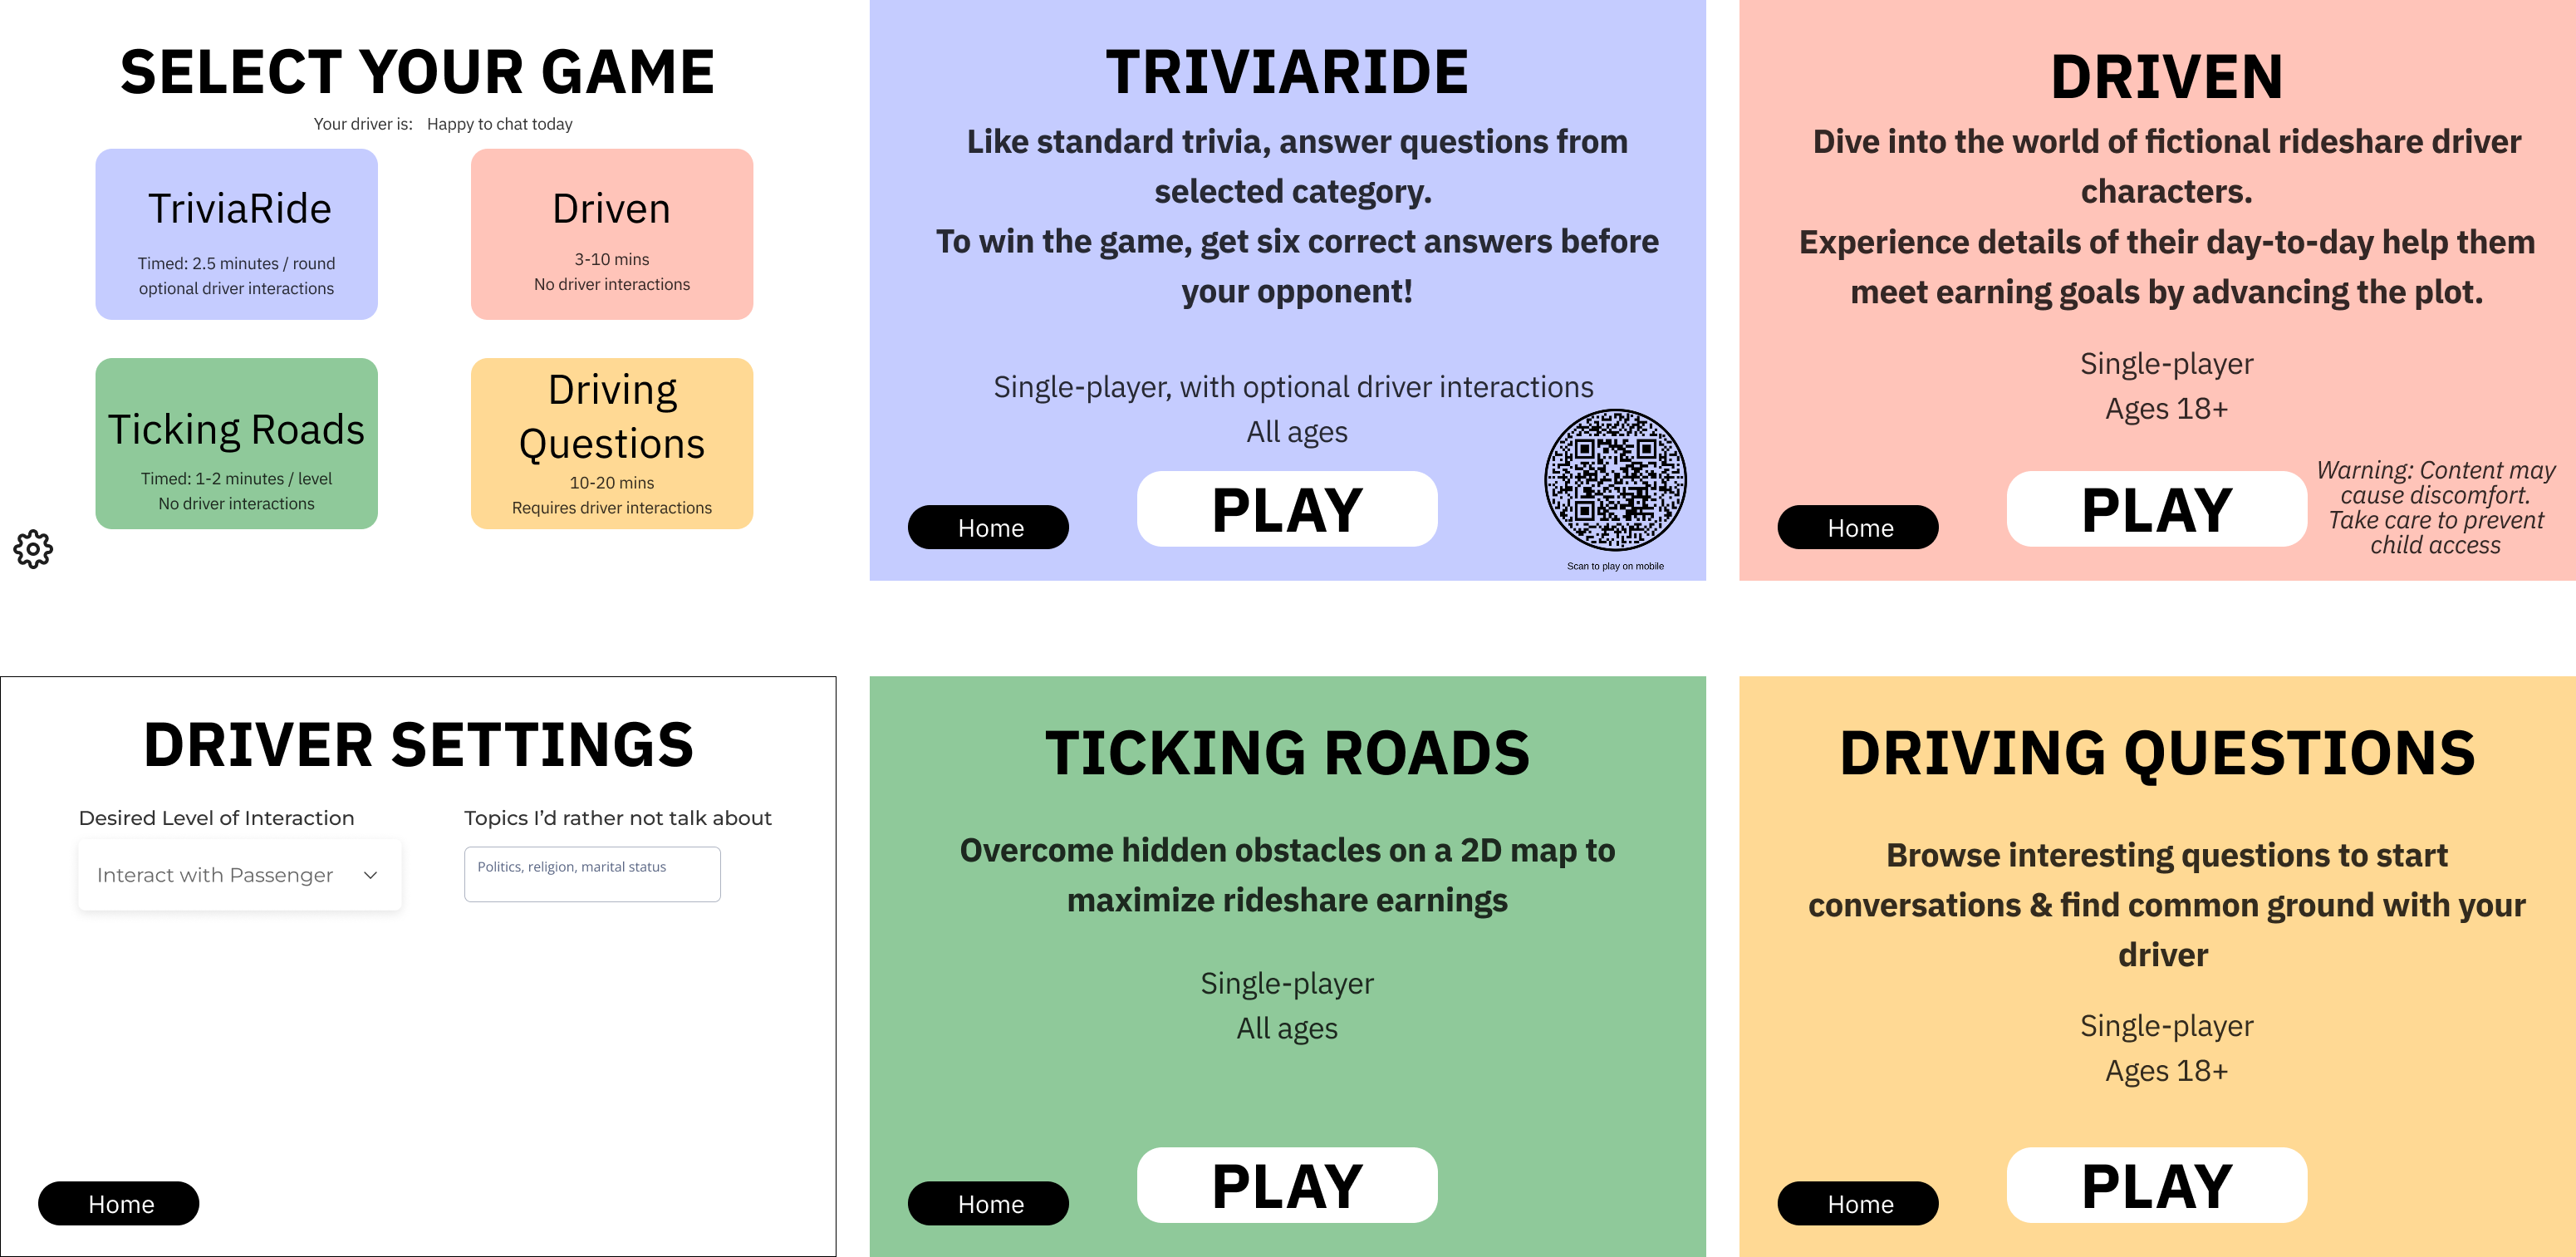
\includegraphics[width=.9\linewidth]{Chapters/figures/menu.png}
    \caption{Menu selection enables passenger selection of games with driver-preference awareness}
    \label{menu}
\end{figure}
\FloatBarrier

\subsection{CrossRoads} 
% \todo{Sophia}
CrossRoads is a standard crossword puzzle that includes clues related to ground-truth rideshare driving concepts. Unlike traditional forms of crossword, drivers have agency to pick and define their own terms and clues to include in their own instances of the game.

\FloatBarrier
\begin{figure}[h!]
    \centering
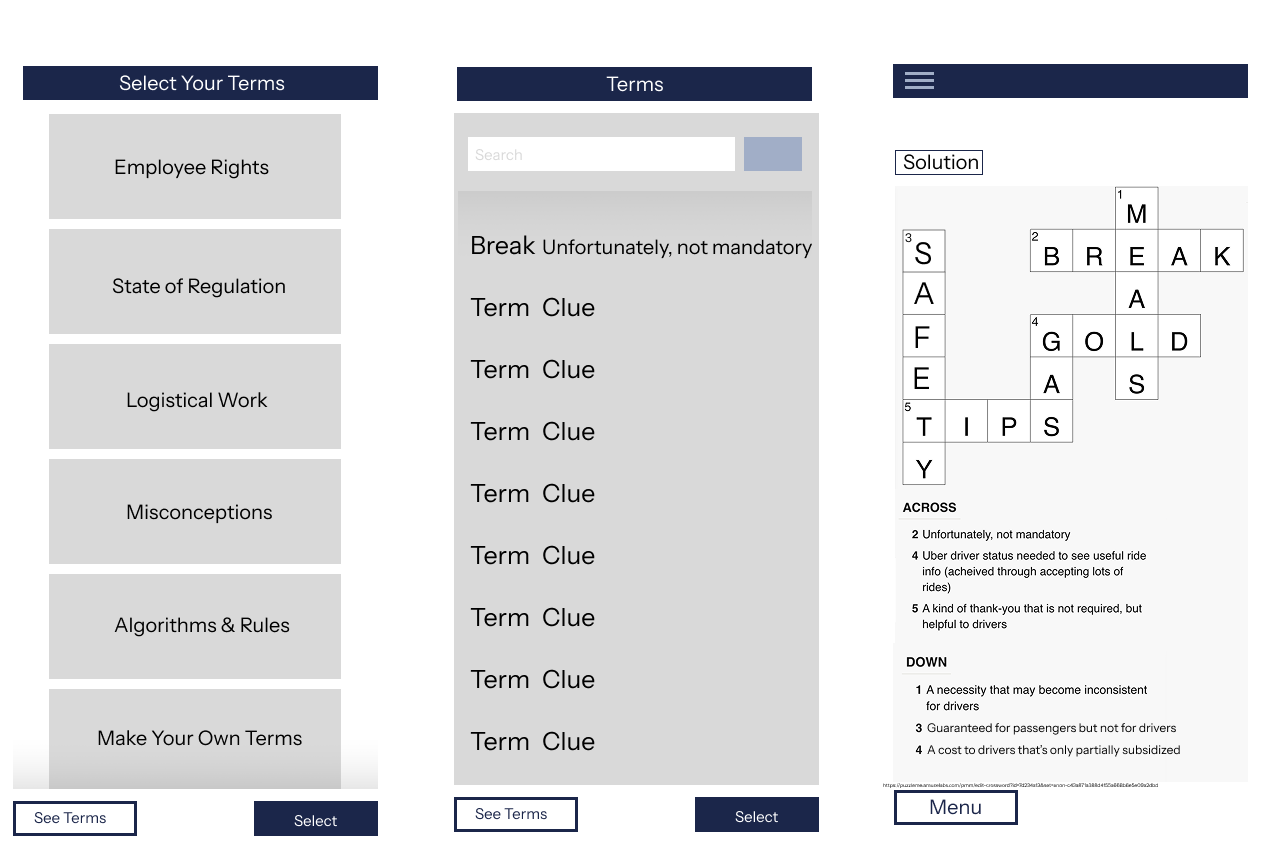
\includegraphics[width=.9\linewidth]{Chapters/figures/CrossRoads.png}
    \caption{CrossRoads contains driver-selected rideshare concepts}
    \label{crossroad}
\end{figure}
\FloatBarrier


\subsection{Dilemmas @ Work} 
% \todo{add visual aid, use figure captions to discuss mechanisms/meanings behind cards}
Based off of the popular social party game \textit{Cards Against Humanity} and inspired by related applications of the card game towards discussion of contexts such as AI ethics \cite{license}, as well as drivers-led advocacy \cite{cards}, we adapted card decks so that black cards represented work dilemmas that drivers and traditional workers might face in their everyday labor -- leveraging intermixing (\S\ref{intermix}). Correspondingly, white cards depicted potential strategies for handling the various dilemmas presented in black. Designed for a physical social context, the random dealing of cards each round creates a replayable (\S\ref{replayable}) experience even among the same group of players.

\FloatBarrier
\begin{figure}[h!]
    \centering
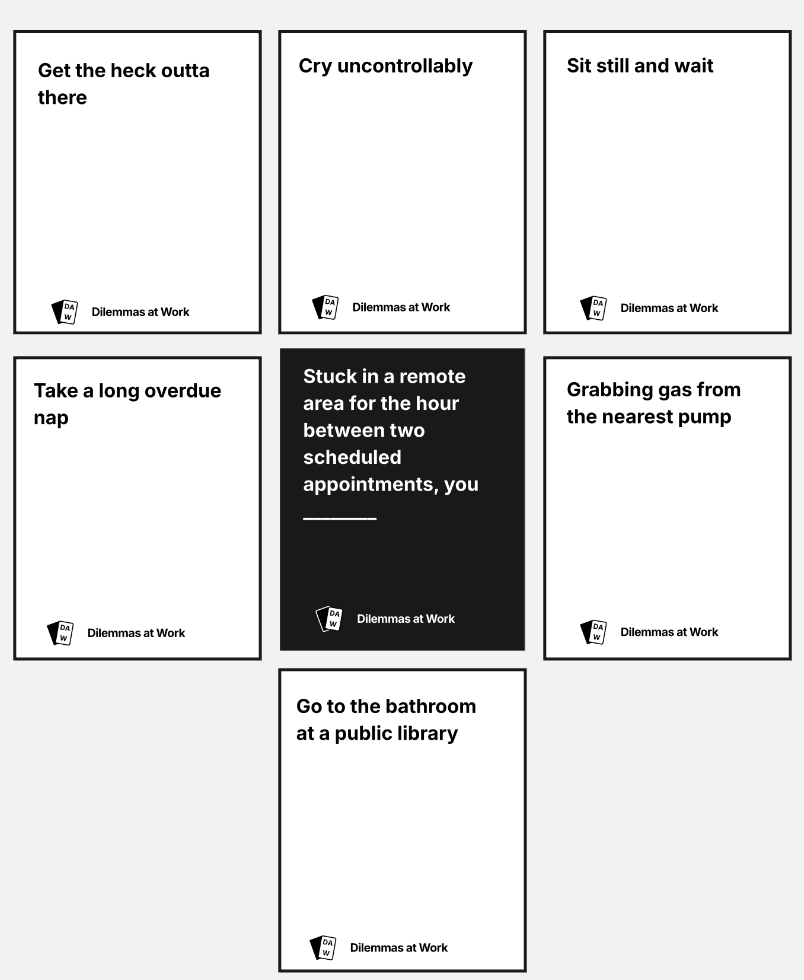
\includegraphics[width=.5\linewidth]{Chapters/figures/Dilemmas.png}
    \caption{Dilemmas @ Work adapts Cards Against Humanities deck where black cards represent worker dilemmas and white cards represent potential tactics in response}
    \label{crossroad}
\end{figure}
\FloatBarrier

\subsection{Driven} 
% \todo{Jose}
The visual novel used feedback we gathered from the first participants who said they wanted something low-impact and casual, but were still drawn to an engaging story.  The visual novel started with one story that centered around a few decisions a driver would have to make in both earning money through the app and in their own life. The story follows David Luiz, a father who was recently laid off from his job who starts ridesharing to make ends meet. The player is able to tap and select 1 of 2 options similarly to a choose-your-own-adventure novel. This game deeply centers around the work-life balance that is often a struggle while ridesharing 

\FloatBarrier
\begin{figure}[h!]
    \centering
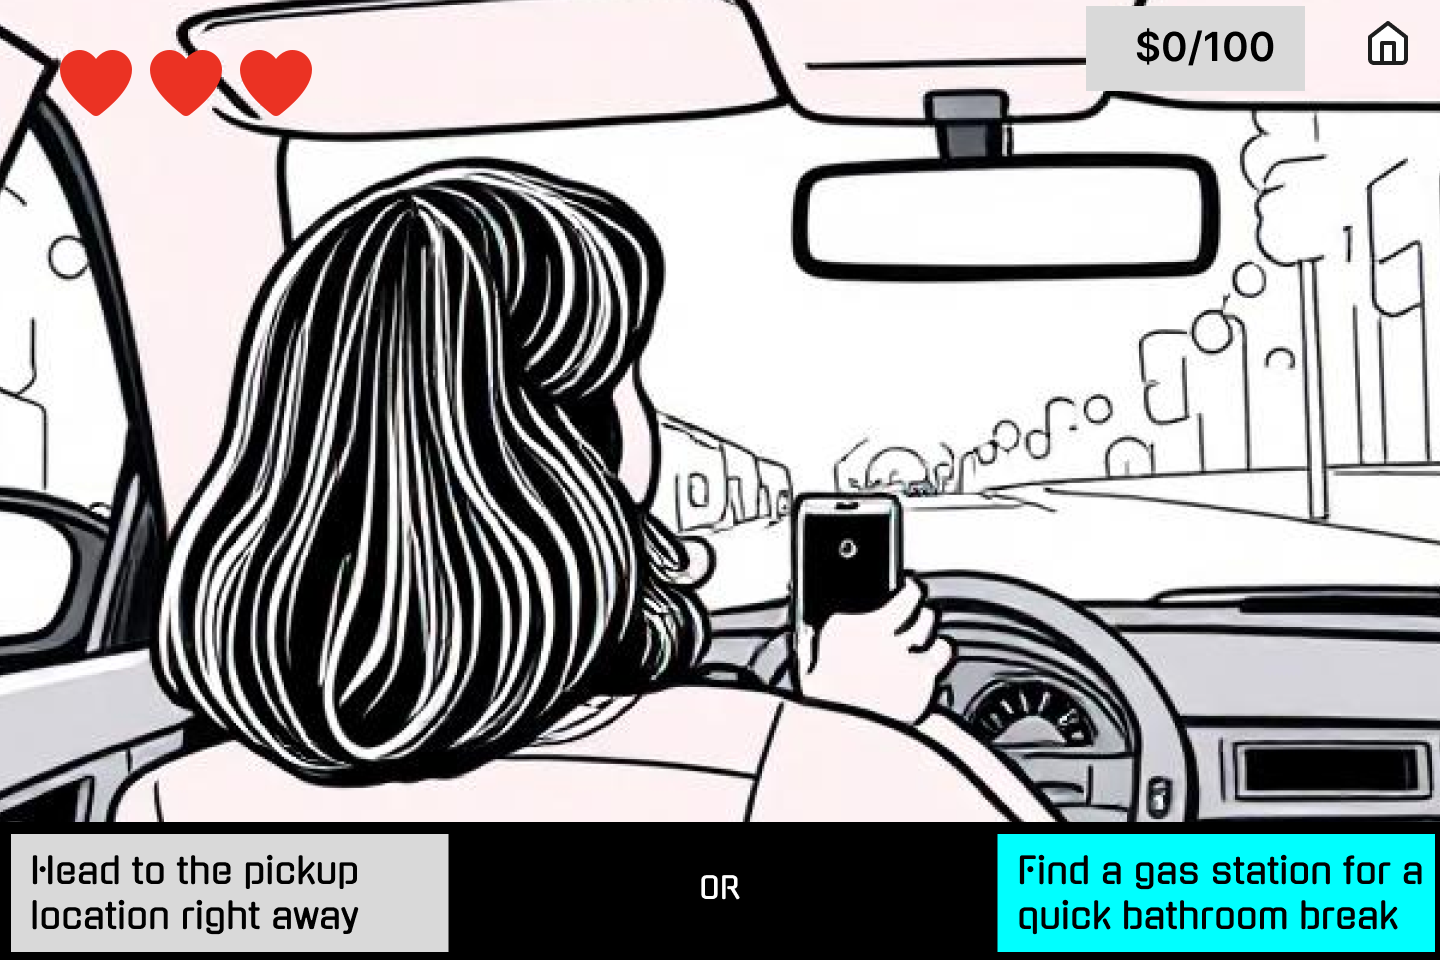
\includegraphics[width=.7\linewidth]{Chapters/figures/driven.png}
    \caption{Driven is visual novel with point-and-click options that advance plotline of two rideshare characters}
    \label{crossroad}
\end{figure}
\FloatBarrier


\subsection{TriviaRide} 
% \todo{Emmie}
After pilot interviews we focused on the games best received both for their gameplay styles and ability to have rideshare concepts embedded. The first prototypes we made were of a categorized trivia game and a narrative visual novel. The trivia game consisted of four categories: Social Studies, Science, Pop Culture, and the Arts. The player of the game is free to choose whichever category they would like, and answer the question that comes after. The game is played against a hypothetical opponent with the goal being the first player to get to 6 correct answers.
The game contained questions regarding the policies and platform information relating to rideshare driving such as “What law classified drivers as independent contractors in CA?” as well as unrelated questions that are more rooted in general trivia. The intermixing allows the game to feel like it's still playful and approachable for every user without the rideshare concepts becoming overwhelming.

\FloatBarrier
\begin{figure}[h!]
    \centering
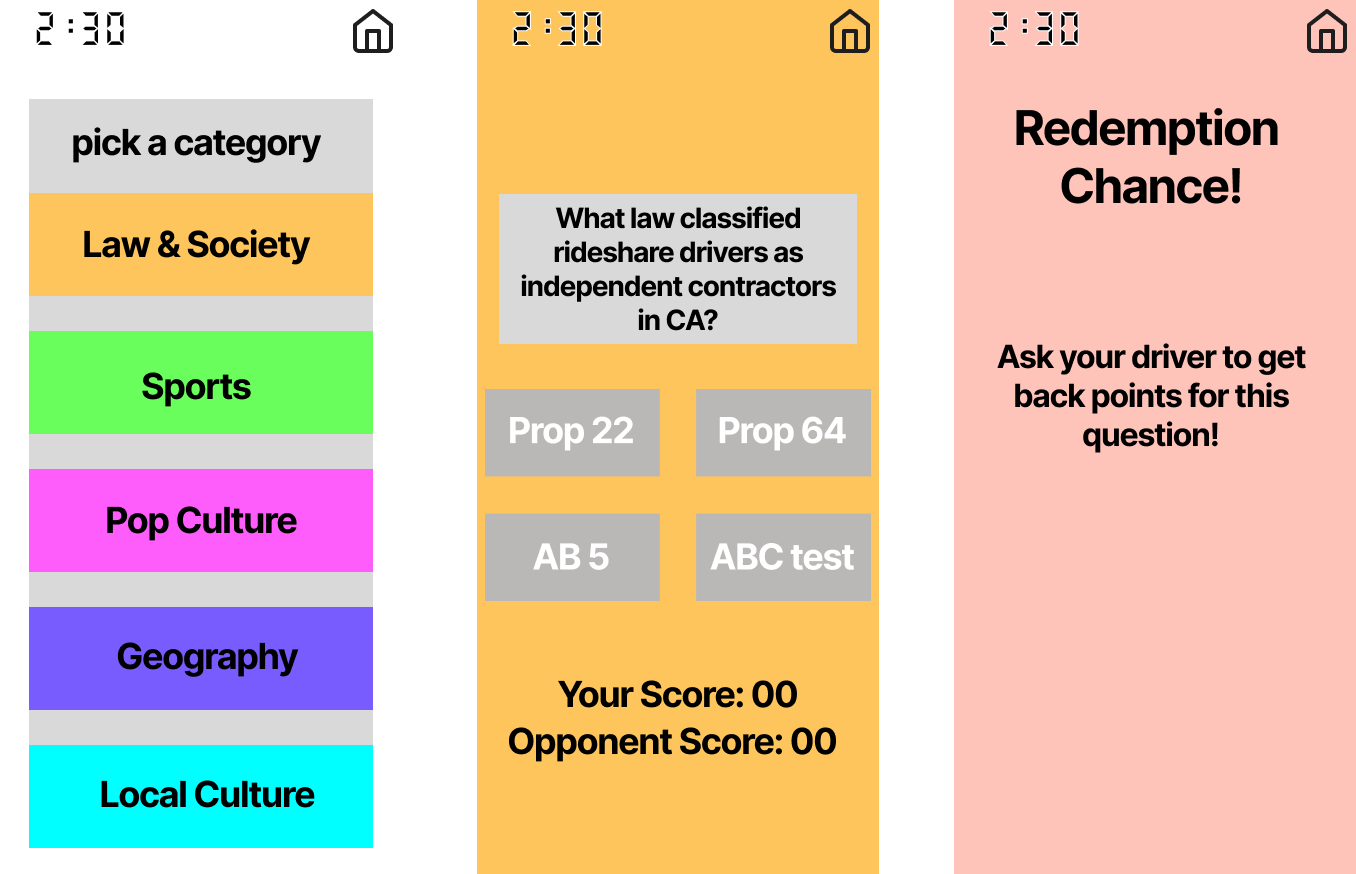
\includegraphics[width=.7\linewidth]{Chapters/figures/triviaRide.png}
    \caption{TriviaRide is a timed challenge with optional driver interactions and embedded rideshare concepts}
    \label{crossroad}
\end{figure}
\FloatBarrier

\subsection{Driving Questions} \label{questions}
 % \todo{someone with time}
Inspired by the game \textit{We’re Not Really Strangers} (WRNS), \textit{Driving Questions} was implemented based on a D1.2's desire to have more interaction between the driver and passenger on an emotional level. WNRS is a conversation prompting game where the player takes turns asking and answering questions. Driving questions serves as boundary object to mediate conversation between drivers and riders, keeping conversations related to the driving conditions while allowing the rider and driver to get to know each other as people. We repeatedly updated the content to arrive at less intrusive, as well as more locally grounded and clear questions.
Ticking Roads fulfills replayable criteria and intermixed embedded design. The game has a limited selection of questions, but because it is conversational, the responses will be different each time with different passenger/driver combinations. 
% Intermixing – some questions are related to rideshare driving – “How do Quests/Challenges work?” while others are broader “What’s your favorite restaurant in the area?”
Concepts embedded included mental health impact, platformic logistics, take rate.

\FloatBarrier
\begin{figure}[h!]
    \centering
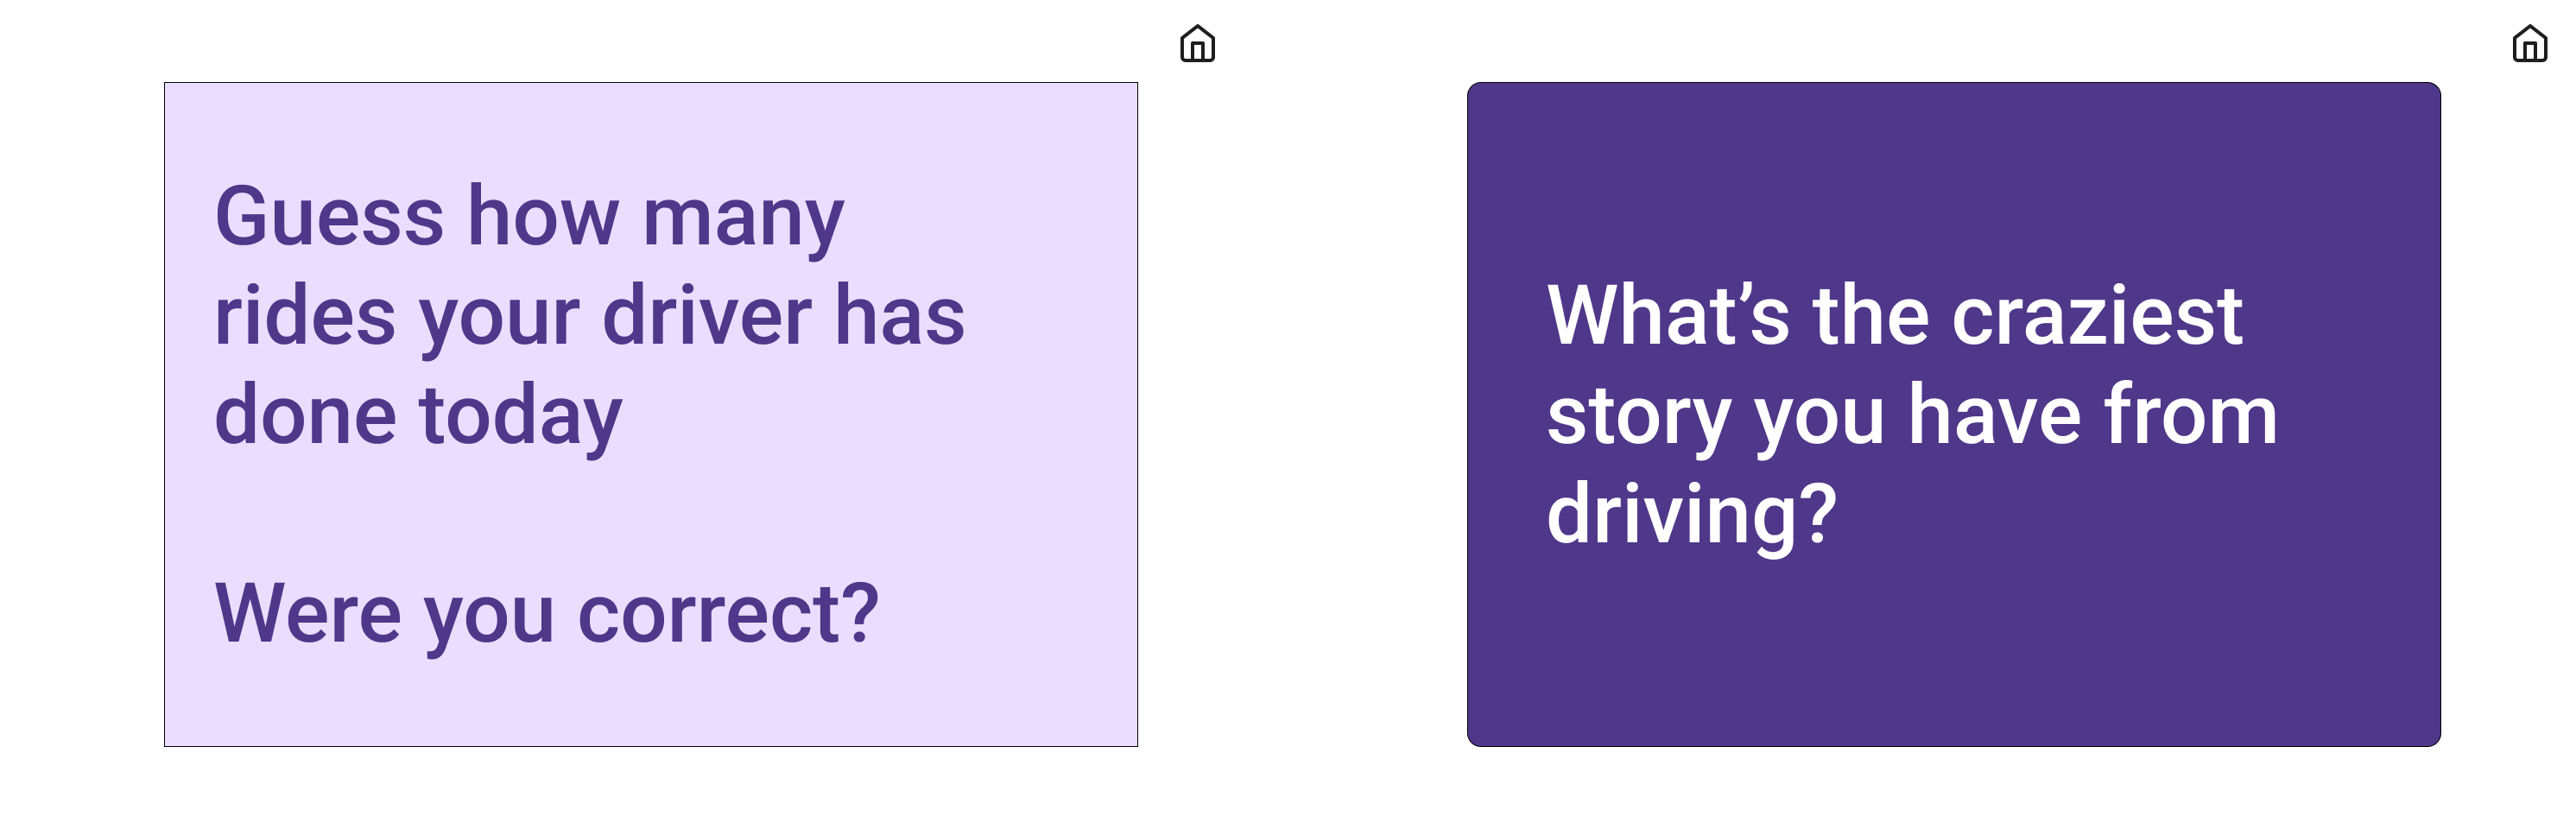
\includegraphics[width=.7\linewidth]{Chapters/figures/questions.png}
    \caption{Driving Questions attempts to bridge the rider-driver social gap with conversation prompts for both sides}
    \label{crossroad}
\end{figure}
\FloatBarrier

\subsection{Ticking Roads} 
% \todo{Jane}
Ticking Roads is a time management game that surfaces stressors of the road to players through obstacles on a map. Players tasks to pick up passengers at designated locations on the map, and receive feedback when performing actions to deal with such tasks (e.g., move around, speeding up/down, waiting at pick up location).
\FloatBarrier
\begin{figure}[h!]
    \centering
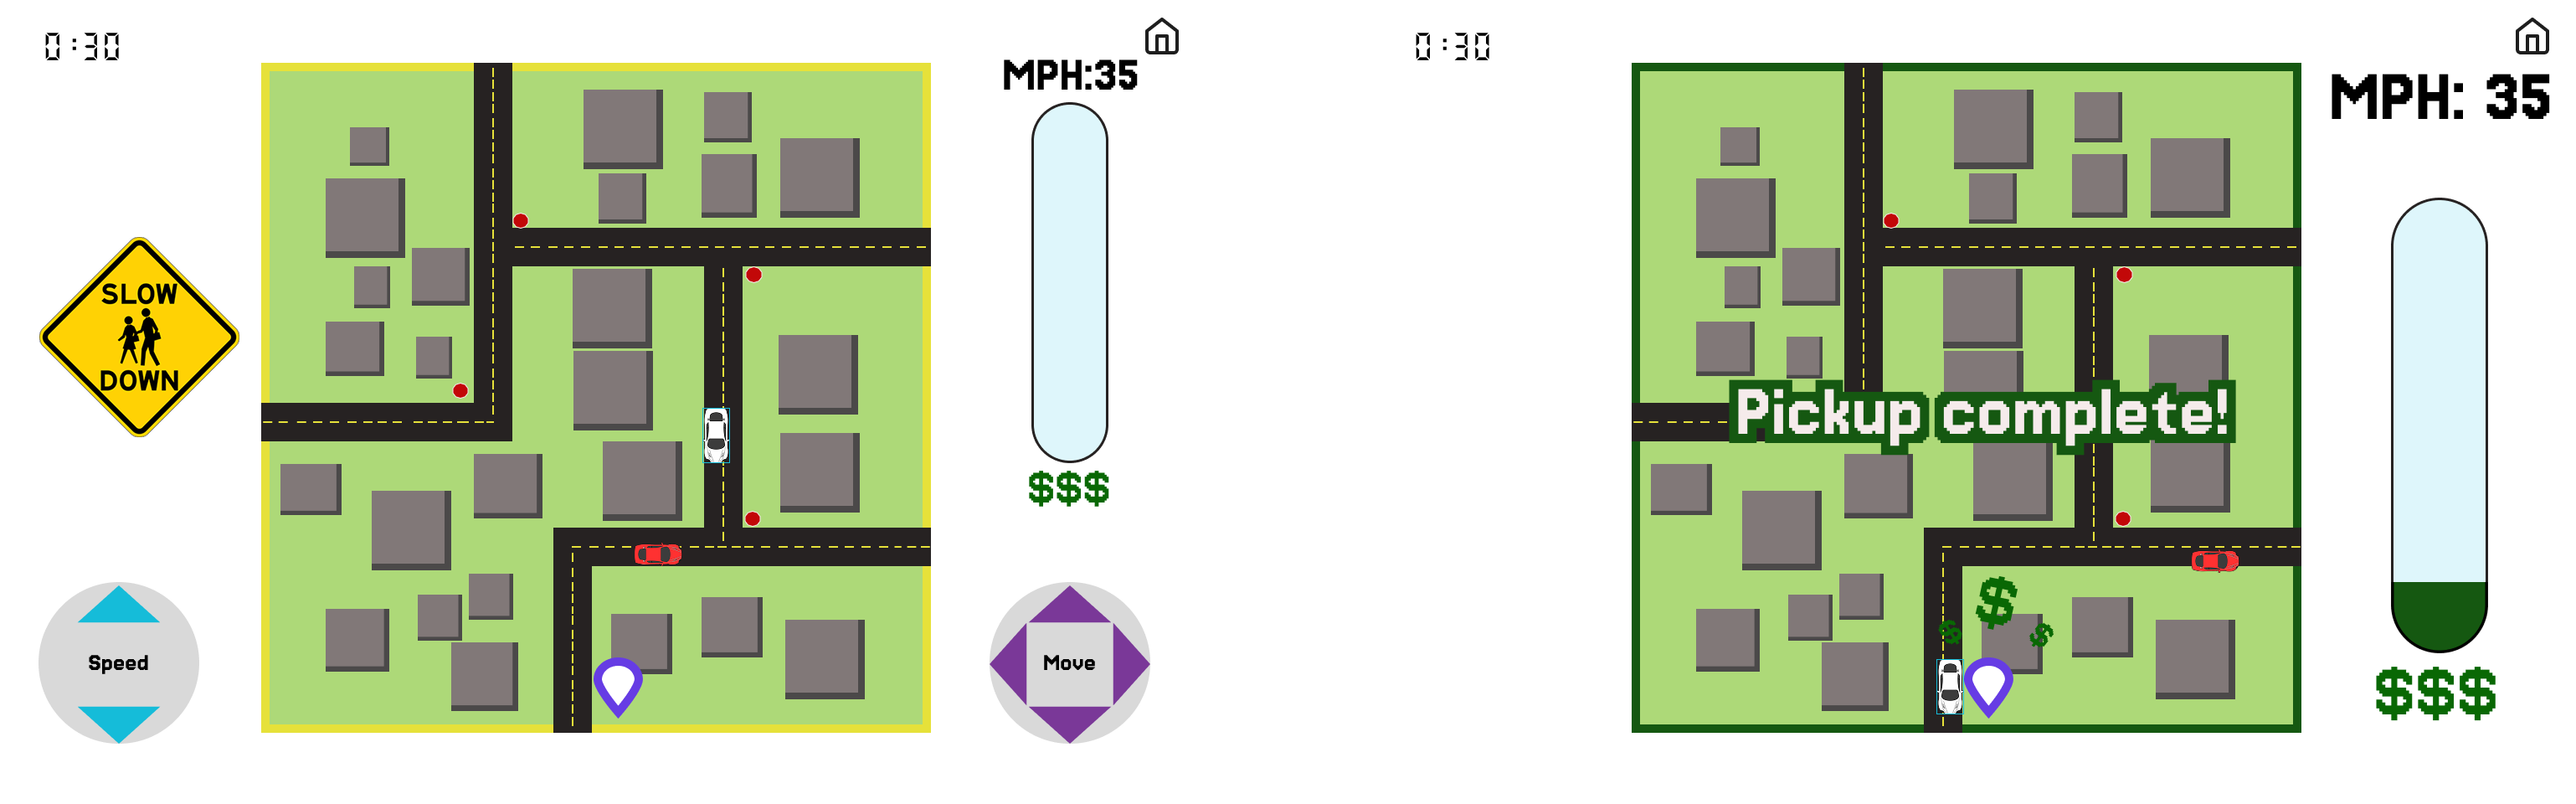
\includegraphics[width=.9\linewidth]{Chapters/figures/ticking.png}
    \caption{TickingRoads simulates rider pickup (logistics) and immediate feedback from controlling car on map}
    \label{ticking}
\end{figure}
\FloatBarrier

\section{Results}

\subsection{Consumer Knowledge Gaps \& Drivers' Prioritized Concepts} \label{pay}
Here we selectively report the most prominent themes that drivers and passenger participants of this workshop brought up, but other forms of covert logistical, emotional and immaterial labor are present, including vehicle-related responsibilities such as gas, oil changes and general car maintenance or in-ride labor to keep the temperature and mood comfortable, as well as the ride itself safe and stable \todo{find PIDs}. We discuss in 6.2 how gamified interactions can assist drivers with service-oriented responsibilities inside the vehicle during rides.

% Drivers communicated a variety of rideshare
\subsubsection{Pay rates} 
A wide variety of stressors plague the daily operations and well-beings of drivers, but none 
surpassed pay in terms of prioritized topics to communicate to riders.
Drivers described rampant passengers misconceptions around pay rates. For instance, driver \todo{find participant id's} relayed how many ``\textit{think that, if the fare is \$100 that we make \$85}'' or how ``\textit{everybody has a 30\% number in their head of what Uber takes, [\dots] which is just simply not the case}'' and
D3.2 would ``\textit{love [passengers] to know that I don't really get the full fare they are paying. [\dots] Uber first of all, take their cut, then I cover fuel, car maintenance, time -- all these are swallowed by [what's broadly considered] service.}''
As a result, passengers are disincentivized to tip: ``\textit{they assume a lot of times that they don't have to tip [\dots] they feel like their charge all goes to the driver}''. 
D1.1 explains how pay overshadows other concerns since adequate compensation may alter their perception of all other stressors they experience: ``\textit{If we are investing our energy, our time, our efforts, frankly, we just don't [want] a feeling of being taken advantage of [\dots] of being manipulated [\dots] of being not cared about. I want to feel like somebody gives a [expletive] about me for the energy I'm putting in, [like] I'm making the money I'm making.}''

% I'd love them to know that I don't really get the full fare they are paying [\dots] A lot of people really think I'm getting all that money that pops up on their app when and they're making that booking. But I'm not. Uber first of all, take their cut, then I cover fuel, car maintenance, time -- all these are swallowed by [what's considered] service. In other words, so if you ever wonder why drivers care about tips or cancellations, that's why, because the money that you pay for the driver or for the service, it doesn't get to me full amount the way it is. Sometimes, after all, the deductions, I'm left with less than half the amount. So it's really tragic. Another thing, I don't get paid to wait at pickups, like I said before, I when you keep me waiting like 5-10 minutes, I'm not really getting paid for that time.‚

Corroborating driver observations, passengers (e.g., all members of PW1 \& PW3) were also ``\textit{surprised about the 30\% [take-home rate our drivers estimated.] I didn't realize that it could be that low. That's bad.}'' In the case of a more sympathetic rider who has asked drivers about rising take rates, P2.2 observed how ``\textit{all the drivers are anxious to answer [\dots to ensure] riders know that even though [passengers] are paying more, [drivers] are not making more}''. 


\subsubsection{Pickup Logistics} \label{pickup}
One overlooked factor impacting pay is the time that drivers spent waiting for passengers during pickup. Drivers such as D3.2 discussed the consequences that pickup delays carry for earnings:
``\textit{I don't get paid to wait at pickups, [\dots] when you keep me waiting like 5-10 minutes, I'm not really getting paid for that time [\dots] that's time and fuel I'm losing, with little or no extra pay.}'' Besides financial losses,  \todo{PID} details how platform mechanisms fall short in ensuring timeliness of passenger arrival: ``\textit{I'm sure the customer doesn't really pay that much more in wait time [\dots] it's not enough to be prohibitive. [\dots] It's almost like they encourage like [platforms] want to encourage that}'', while P3.3 ``\textit{second[s] that the waiting time is really expensive, especially when gas prices go up [\dots] depending on what car we're using to drive it could just eat into our profits }so bad\textit{, and I feel like only us drivers really understand that.}'' Other road conditions such as parking availability also impact drivers during pickup, P1.2 describes a time when 
\begin{quote}
    ``\textit{I had to pick up someone, it was center of the city, and there's literally is no parking, it's red lanes on both sides -- bus only lanes. You can't drive in those lanes. You can't stop, you can't park, you literally just can't be in those lanes. So I was sitting in that lane waiting [and] of course, the bus came through. I got a ticket.}''
\end{quote}

Passengers also expressed curiosity around pickup mechanisms. P3.3, for instance, wonders and worries about how their suburban location impact driver earnings  ``\textit{I live in a suburb \dots and I always wonder, if they're  \dots having to drive so far to each location to drive people around, I don't think they're getting paid between the different ones. \dots I always wonder if they're making a lot less money and just driving basically for free between the places.}'' Relatedly, P3.3 then considers how location affects driver arrival time and her own passenger ratings: ``\textit{they come really early sometimes. And I always wonder, do they mark off if you don't come right out? If we say, come at 5pm and they come in 4:45pm, and we don't come out, I wonder if they mark off [my passenger ratings]. Because well, it's not my fault.}''

\subsubsection{Rating Pressures \& Passenger Expectations of Service} \label{ratings}
Driver ratings constitute another notable variable that exerts psychological control in rideshare labor, since drivers with ratings under certain thresholds may experience platforms' elimination through deactivation \cite{free}. 
% are pressures to keep ratings above a threshold
However, passengers with high expectations and little awareness around the harsh effects of ratings will often ``\textit{give low ratings for things out of my control -- e.g., traffic delays, being in a rush, or even misunderstandings over route choices -- so ratings feel personal, but the reality is more complicated}'' (D3.1). However, drivers point to a plethora of factors, stressors and costs that remain unobservable to passengers, and such invisibility drives up their expectations of service and rating pressures: 

\begin{quote}
    ``\textit{Ratings can drop for stuff I can't control, and sometimes I'm reading the vibe and giving folks their space, not just ignoring them. We are not just driving, we are juggling through navigation, personalities and keeping things safe. The app itself is not perfect, it doesn't show everything we are dealing with, so [passengers] should be a little bit more understanding}.''
\end{quote}


\subsection{Consent \& Content in Gamified Rideshare Interactions}

\subsubsection{Overcoming Driver-Rider Social Boundaries} Both riders and drivers expressed inherent hesitancy to initiate conversation. Up front, drivers feared putting customers on the spot since ``\textit{not every rider wants to interact. And if the game feels too personal or like a distraction from driving, it can backfire}'' (\todo{DW3}), approaching overly heavy or suggestive topics such as ``\textit{sexually suggestive or flirty questions? No, no, not, not the place [\dots] It's gross, it's unsafe, and it creates a very dangerous precedent, especially for for women drivers and riders}'' (D2.2). In the backseat, passengers observed and respected drivers' rating pressures that compels them to keep riders comfortable in terms of conversation topic, noting how ``\textit{in a car there is that dynamic of: they don't want to make you feel uncomfortable, and if I just bring up a topic that makes them feel uncomfortable, I don't think that [helps]}'' (P2.3), and acknowledging ``\textit{a fine line between having a genuine interest and prying [\dots] as passengers, we have to be conscious of the fact that these drivers don't want to offend us, because after all, their rating is at stake, so questions should not be intrusive}'' (P2.2).

\ul{Driving Questions} presents an opportunity to bridge the social boundary between drivers and riders. For instance, P3.3 identified as ``\textit{an introvert [\dots] and I have trouble starting conversations [\dots] but it's something this game would help me be more talkative, because it gives me things to say}''. However, the opportunity to bridge the social barrier also introduce risks of intruding privacy. For example, discussions about pay (a prioritized topic by drivers -- \S\ref{pay}) makes passengers such as P3.1 ``\textit{feel uncomfortable asking them how much they're getting paid, or their take home pay}'', let alone more personal inquiries about what drivers miss (\ref{questions}), since ``\textit{it can be painful when you leave your home country}'' (P2.2).

\subsubsection{Balancing Lighter Logistics \& Heavier Labor Topics}
Passengers took care to minimize belittling or criticizing of drivers. For instance, self-conscious riders such as P1.2 ``\textit{don't really feel that it's like right for me to criticize the way they're doing their job, because I don't really know anything about what it's like being a rideshare driver}'', while P2.2 recognized the power differential they held over drivers: ``\textit{it is important that we recognize what our position is in the rideshare thing, and we don't offend people or put them on spots}''.
Despite the hesitation to upset drivers, passengers felt comfortable discussing more rideshare-specific logistics, including the number of rides the driver has completed or reasons for cancellations (P3.3), time spent between rides (P2.2), or how ratings compare to those of other service platforms (P2.3).

For heavier topics, the visual novel was effective at presenting heavy and thought-provoking topics (e.g., harassment or family obligations) in creative and memorable ways (D2.2, D3.1), but also runs the risk of being too long or heavy for the ride. Thus, even though passengers found the visual novel thought-provoking (P1.4, P2.4, P3.2, P1.4) and ``\textit{fun to play in the backseat [\dots] I was pretty invested}.'', others found it ``\textit{emotionally taxing}'' and ``\textit{frighteningly realistic}'' (P2.4) -- making drivers
``\textit{worry about it being too much for some passengers, [since] not everybody [is] in the mood for deep [content] or or even hearing stories}'' (D2.2).

Drivers also recognized the potential for games like \textit{Driven} to engage passenger attention, alleviating their immaterial/emotional labor to keep passengers entertained. Drivers such as D3.1 described combinations of immaterial labor involved, many of which still resemble those found a decade back by \citet{immaterial}: \
\begin{quote}
  ``\textit{There's always a bit of emotional effort in every ride [\dots] [when] I'm not just driving. I'm paying attention to your body language, your tone, your energy, from the moment you get [in] [\dots] If you're if you're chatty, I'll match that. If you're quiet or stressed. I'll try to keep things calm and give you space so it's little things -- e.g., adjusting the music so it fits your mood, making sure the temperature is comfortable, choosing the smooth test route so you're not bouncing around in the back}'' 
\end{quote}
D3.2 also shared how engaging games can alleviate the emotional labor that he performs by distracting their attention from factors like traffic or other time pressures:  ``\textit{it passes time fast, also especially helpful on short trips or when we are stuck in traffic, riders stop checking how long it's taking}.''
% \begin{itemize}
    % \item \textit{Driving Conversations} can break barriers to start connection but trades off with potential of intruding on privacy
    % \item Visual novel \textit{Driven} introduce thought-provoking topics but heavy and possibly time-consuming
    % \item social boundaries and power differentials between drivers and passengers
    % \item gamified interactions mediating as a boundary object
%     \item 
% \end{itemize}

\section{Discussion}

More than a decade ago, \citet{kitturfuture} posed the question of whether we can ``foresee a future a crowd workplace in which we would want our children to participate?'' Borrowing this lens of envisioning and creating healthier (gig) workplaces for posterity, this study approaches improved working conditions for rideshare driving through game design as a medium to (1) challenge and contest existing conditions by proposing alternative futures and (2) engage the younger ridership demographic, many of who may benefit from knowledge about the various responsibilities of rideshare driving --- e.g., financial/algorithmic literacy, asset management, car maintenance.

Through a ``soft action'' like gamified interactions presented in our prototypes, we explore how ``can we activate'' and mobilize methods in design, to enact change related to a disruptive technology \cite{considerations}.
By engaging consumers in the labor advocacy process, we can begin opening up opportunities for end-user audits \cite{eu_audits} or collective resistance through non-use tactics \cite{non_use}. Additionally, we surfaced opportunities for new interactions and incentives that can promote more aligned and mutually beneficial interactions and understandings between drivers and riders.
